\documentclass{beamer}
\usepackage{tikz,amsmath,hyperref,graphicx,stackrel,animate,tipa}
\usetikzlibrary{positioning,shadows,arrows,shapes,calc}
\newcommand{\ipa}[1]{\textipa{#1}}
\newcommand{\argmax}{\operatornamewithlimits{argmax}}
\newcommand{\argmin}{\operatornamewithlimits{argmin}}
\mode<presentation>{\usetheme{Frankfurt}}
\DeclareMathOperator*{\softmax}{softmax}
\AtBeginSection[]
{
  \begin{frame}<beamer>
    \frametitle{Outline}
    \tableofcontents[currentsection,currentsubsection]
  \end{frame}
}
\title{Lecture 11: Discriminative vs.~Bayesian Classification}
\author{Mark Hasegawa-Johnson\\All content~\href{https://creativecommons.org/licenses/by-sa/4.0/}{CC-SA 4.0} unless otherwise specified.}
\date{ECE 417: Multimedia Signal Processing, Fall 2020}  
\begin{document}

% Title
\begin{frame}
  \maketitle
\end{frame}

% Title
\begin{frame}
  \tableofcontents
\end{frame}


%%%%%%%%%%%%%%%%%%%%%%%%%%%%%%%%%%%%%%%%%%%%
\section[Review]{Review: Neural Network}
\setcounter{subsection}{1}

\begin{frame}
  \frametitle{Review: Neural Network}
  Let's review how a neural net works.  Suppose we have a net with two
  layers, whose weight matrices are
  \begin{displaymath}
  W^{(1)}=
  \left[
    \begin{array}{cc}
      2&-1\\0&1
    \end{array}
    \right],~~~
  W^{(2)}=
  \left[
    \begin{array}{cc}
      -0.1&0.03\\0.2&0.05
    \end{array}
    \right]
  \end{displaymath}
  and with no bias vectors.  Suppose it uses ReLU nonlinearity in the
  hidden layer.

  As in Faster-RCNN, let's suppose that the two different outputs are
  treated in two different ways:
  \begin{enumerate}
  \item The first element of the output
  vector, $\hat{y}_0$, is a regression output: no output nonlinearity.
  Loss function is MSE if the classification target is 1 ($y_1=1$), otherwise
  the loss is zero.
  \item The second element of the output vector, $\hat{y}_1$, is a
  classification output: sigmoid nonlinearity, scored with binary
  cross entropy.
  \end{enumerate}
\end{frame}

\begin{frame}
  \frametitle{Neural Network Example}
  Let's suppose we have a minibatch with just one training token:
  \begin{displaymath}
    \vec{x}=[4,1]
  \end{displaymath}
  Suppose that the regression target (the first output target) is
  $y_0=0.4$, and the classification target (the second output target)
  is $y_1=0$ (i.e., no object is present), so that
  \begin{displaymath}
    \vec{y}=[0.4,0]
  \end{displaymath}
\end{frame}

\begin{frame}
  \frametitle{Forward Pass: First layer}

  Suppose the input vector is
  $\vec{x}=[4,1]$.  The hidden layer excitation is
  \begin{displaymath}
  \vec{e}^{(1)} = \vec{x} W^{(1)}=[4,1]\left[\begin{array}{cc}2&-1\\0&1\end{array}\right]=[8,-3]
  \end{displaymath}
  The hidden layer activation is
  \begin{displaymath}
  \vec{h}=\mbox{ReLU}\left(\vec{e}^{(1)}\right)=[8,0]
  \end{displaymath}
\end{frame}

\begin{frame}
  \frametitle{Forward Pass: Second Layer}

  The second layer excitation is
  \begin{displaymath}
  \vec{e}^{(2)}=\vec{h}W^{(2)}=[8,0]\left[\begin{array}{cc}-0.1&0.03\\0.2&0.05\end{array}\right]
  = [-0.8, 0.24]
  \end{displaymath}
  The activation function is linear for the first output, but sigmoid
  for the second output:
  \begin{displaymath}
  \hat{y}=\left[-0.8, \frac{1}{1+e^{-0.24}}\right] =
  \left[-0.8, 0.56 \right]
  \end{displaymath}
\end{frame}

\begin{frame}
  \frametitle{Loss Function}

  Remember that the target is $\vec{y}=[0.4,0]$, and the network
  output is $\hat{y}=\left[-0.8, 0.56 \right]$.  The first output,
  $\hat{y}_0$, is scored using mean squared error if $y_1=1$,
  otherwise it is not scored at all, thus
  \begin{displaymath}
    {\mathcal L}_r = y_1\frac{1}{2}\left(y_0-\hat{y}_0\right)^2 =
    0\times \frac{1}{2}\left(-0.8-0.4\right)^2 =0\times 0.72 = 0
  \end{displaymath}
  The second output, $\hat{y}_1$, is scored using binary cross
  entropy, thus
  \begin{displaymath}
    {\mathcal L}_c = -\left(y_1\ln\hat{y}_1+(1-y_1)\ln(1-\hat{y}_1)\right)
    = -\ln(1-0.56)
  \end{displaymath}
\end{frame}

\begin{frame}
  \frametitle{Backward Pass: Second Layer}

  Both BCE and MSE have the same simple form for the output-layer loss
  gradient:
  \begin{displaymath}
    \nabla_{\vec{e}^{(2)}}{\mathcal L}=
    \left(\hat{y}-\vec{y}\right)
  \end{displaymath}
  But the first term (the regression loss) is scored if and only if
  $y_1=1$.  Since, in our example, $y_1=0$, we have
  \begin{displaymath}
    \nabla_{\vec{e}^{(2)}}{\mathcal L}
    = [0\times(-0.8-0.4), (0.56-0)]=[0, 0.56]
  \end{displaymath}
\end{frame}

\begin{frame}
  \frametitle{Backward Pass: First Layer Activations}

  The derivative of loss with respect to the first-layer activations
  is obtained by back-propagating from the second-layer, which is just
  multiplying by the transpose of the weight matrix:
  \begin{displaymath}
    \nabla_{\vec{h}}{\mathcal L}=
    \nabla_{\vec{e}^{(2)}}{\mathcal L}W^{(2),T}.
  \end{displaymath}
  In our example,
  \begin{displaymath}
    \nabla_{\vec{h}}{\mathcal L}=    
          [0,0.56]\left[\begin{array}{cc}-0.1&0.2\\0.03&0.05\end{array}\right]    =
          [0.0168,0.028]
  \end{displaymath}
\end{frame}

\begin{frame}
  \frametitle{Backward Pass: First Layer Excitations}

  The first-layer excitation gradient is is obtained by multiplying
  the activation gradient by the derivative of the nonlinearity.  
  \begin{displaymath}
    \nabla_{\vec{e}^{(1)}}{\mathcal L}=
    \nabla_{\vec{h}}{\mathcal L}\odot \frac{\partial h}{\partial e^{(1)}}
  \end{displaymath}
  In the case of ReLU, the derivative is either $0$ or $1$, so
  \begin{displaymath}
    \nabla_{\vec{e}^{(1)}}{\mathcal L}=    
          [0.0168,0.028] \odot [1,0] = 
          [0.0168,0]
  \end{displaymath}
\end{frame}

\begin{frame}
  \frametitle{Weight Gradients}

  The weight gradients are the vector outer products of the
  forward pass and the backward pass:
  \begin{displaymath}
    \nabla_{W^{(1)}}{\mathcal L}
    = \left(\vec{x}\right)^T\left(\nabla_{\vec{e}^{(1)}}{\mathcal L}\right) =
    \left[\begin{array}{c}4\\1\end{array}\right]\left[0.0168,0\right]=
    \left[\begin{array}{cc}0.0672&0\\0.0168&0\end{array}\right]
  \end{displaymath}
  \begin{displaymath}
    \nabla_{W^{(2)}}{\mathcal L}
    = \left(\vec{h}\right)^T\left(\nabla_{\vec{e}^{(2)}}{\mathcal L}\right) =
    \left[\begin{array}{c}8\\0\end{array}\right]\left[0,0.56\right]=
    \left[\begin{array}{cc}0&4.48\\0&0\end{array}\right]
  \end{displaymath}
\end{frame}

\begin{frame}
  \frametitle{Summary}
  \begin{itemize}
  \item Forward-pass is a matrix multiply:
    \[
    \vec{e} = \vec{h}W
    \]
  \item Backward-pass is multiplication by the transposed matrix:
    \[
    \nabla_{\vec{h}}{\mathcal L} = \left(\nabla_{\vec{e}}{\mathcal L}\right)\left(W\right)^T
    \]
  \item Weight gradient is a vector outer product:
    \[
    \nabla_{W}{\mathcal L} = \left(\vec{h}\right)^T\left(\nabla_{\vec{e}}{\mathcal L}\right)
    \]
  \end{itemize}
\end{frame}
     
%%%%%%%%%%%%%%%%%%%%%%%%%%%%%%%%%%%%%%%%%%%%
\section[LVCSR]{Neural network based large vocabulary continuous speech recognition}
\setcounter{subsection}{1}

\begin{frame}
  \frametitle{Speech Recognition: So Far}

  Speech recognition using a nearest-neighbor classifier
  \begin{itemize}
  \item \ldots works very well for isolated-word recognition, in vocabularies
    of up to about ten different words.
  \item \ldots fails\ldots
    \begin{itemize}
    \item \ldots for detection/segmentation.  Nearest-neighbors can't
      tell you where the word started, where it ended.
    \item \ldots for continuous speech recognition.  Nearest-neighbors
      can't transcribe a sequence of words.
    \item \ldots for large vocabularies.  If you want to add a new
      word to the vocabulary, you need to record examples of that
      word; not very scalable, if you want 100k words.
    \end{itemize}
  \end{itemize}
\end{frame}
  
\begin{frame}
  \frametitle{Large-Vocabulary Continuous Speech Recognition (LVCSR)}

  An LVCSR has two components:
  \begin{enumerate}
  \item Acoustic model.  This is a neural net that classifies which
    speech sound is being produced at any given instant.
  \item Pronunciation model + Language model. Converts a sequence of
    speech sounds to a sequence of words.  Three technologies, each requires
    more training data than the last:
    \begin{itemize}
    \item hidden Markov model (HMM)
    \item recurrent neural network (RNN)
    \item attention-based sequence-to-sequence (Transformer)
    \end{itemize}
  \end{enumerate}
\end{frame}

\begin{frame}
  \frametitle{Acoustic Event Detection, Video Event Detection}

  BTW, the same two parts exist in most acoustic event detection (AED) and
  multimedia activity transcription models:
  \begin{enumerate}
  \item Acoustic/Visual model.  This is a neural net that classifies which
    acoustic event/visual event is occurring at any given instant.
  \item Sequence model: arranges atomic acoustic/visual events into
    acoustic scenes or complex events/activity sequences.
  \end{enumerate}
\end{frame}

\begin{frame}
  \frametitle{Large-Vocabulary Continuous Speech Recognition (LVCSR)}

  Today we'll focus on this one:
  \begin{itemize}
  \item Acoustic model.  This is a neural net that classifies which
    speech sound is being produced at any given instant.
  \end{itemize}
  Thursday  we'll focus on this one:
  \begin{itemize}
  \item Pronunciation model + Language model. Converts a sequence of
    speech sounds to a sequence of words:
    \begin{itemize}
    \item hidden Markov model (HMM)
    \end{itemize}
  \end{itemize}
\end{frame}

%%%%%%%%%%%%%%%%%%%%%%%%%%%%%%%%%%%%%%%%%%%%
\section[Phonemes]{Speech sounds: phones and phonemes}
\setcounter{subsection}{1}

\begin{frame}
  \frametitle{Large-Vocabulary Continuous Speech Recognition (LVCSR)}

  Today we'll focus on this one:
  \begin{itemize}
  \item Acoustic model.  This is a neural net that classifies which
    speech sound is being produced at any given instant.
  \end{itemize}
  But what does that mean, ``which speech sound is being produced''?  
\end{frame}

\begin{frame}
  \frametitle{Phonemes}

  A phoneme is
  \begin{itemize}
  \item a speech segment (temporally contiguous) that
  \item can be used to make up new words, but is also used in existing words, and
  \item if you change it to a different phoneme, you can change the
    meaning of the word.
  \end{itemize}
\end{frame}

\begin{frame}
  \frametitle{Phonemes: Example}

  \begin{block}{}
    Who'd heed a gardener who had never hid his head in a hood?  How'd
    you believe him?  Have you heard that he hayed, or hoed, or
    carried a hod, or hied his hoy to HUD?
  \end{block}
  \begin{block}{General American English has 15 vowels, if you count schwa (\ipa{[@]})}
    \begin{scriptsize}
      \centerline{\begin{tabular}{|l|c|c||l|c|c||l|c|c|}\hline
          Example & IPA & ARPA & Example & IPA & ARPA & Example & IPA & ARPA \\\hline
          heed & \ipa{[i]} & IY & who'd &  \ipa{[u]} & UW & heard & \ipa{[\textrhookrevepsilon]} & ER \\
          hid & \ipa{[I]} &  IH & hood & \ipa{[U]} & UH & how'd &  \ipa{[aU]} & AW \\
          hayed & \ipa{[e]} & EY & hoed & \ipa{[o]} & OW & hied &  \ipa{[AI]} & AY \\
          head & \ipa{[E]} & EH & HUD & \ipa{[2]} & AH & hoy & \ipa{[OI]} & OY \\
          had & \ipa{[\ae]} & AE & hod & \ipa{[A]} & AA & a &  \ipa{[@]} & AX \\ \hline
      \end{tabular}}
    \end{scriptsize}
  \end{block}
\end{frame}

\begin{frame}
  \frametitle{Phoneme Notations}

  There are two types of phoneme notations that you should know about
  for this course.
  \begin{enumerate}
  \item The International Phonetic Alphabet (IPA:
    \url{https://en.wikipedia.org/wiki/International_Phonetic_Alphabet}).
    Invented in Europe around 1888.
  \item ARPABET (\url{https://en.wikipedia.org/wiki/ARPABET}) is a
    set of ASCII (plaintext) codes for English phonemes.  Still used
    on systems where unicode support is uncertain.
  \end{enumerate}
\end{frame}

\begin{frame}
  \frametitle{Phonemes: Example}

  \begin{block}{}
    The quick brown fox jumped over the lazy dog.
    
    \ipa{[D@ kwIk b\:RaUn fAks dZ2mpt ov{\textrhookrevepsilon} D@ lezi dAg]}
  \end{block}
  \begin{block}{General American English has 24 consonants}
    \begin{scriptsize}
      \centerline{\begin{tabular}{|l|c|c||l|c|c||l|c|c|}\hline
          Stops \& & IPA & ARPA & Fricatives & IPA & ARPA & Nasals\& & IPA & ARPA \\
          Affricates &  &  &  &  &  & Glides & & \\\hline
          poe & \ipa{[p]} & P & fan &  \ipa{[f]} & F & moo & \ipa{[m]} & M \\
          bo & \ipa{[b]} &  B & van & \ipa{[v]} & V & no & \ipa{[n]} &  N \\
          tow & \ipa{[t]} & T & thin & \ipa{[T]} & TH & sing & \ipa{[N]} & NG  \\
          dough & \ipa{[d]} & D & than & \ipa{[D]} & DH & woe &  \ipa{[w]} & W \\
          cho & \ipa{[tS]} & CH & Sue & \ipa{[s]} & S & low & \ipa{[l]} & L \\
          joe & \ipa{[dZ]} & JH & zoo & \ipa{[z]} & Z & row & \ipa{[\:R]} & R \\
          ko &\ipa{[k]} & K & ship & \ipa{[S]} & SH & yo &  \ipa{[j]} & Y  \\
          go & \ipa{[g]} & G & beige & \ipa{[Z]} & ZH & ho & \ipa{[h]} & HH \\\hline
      \end{tabular}}
    \end{scriptsize}
  \end{block}
\end{frame}

\begin{frame}
  \frametitle{How to use phonemes}

  Phonemes are used:
  \begin{enumerate}
  \item \ldots for detection/segmentation.  Nearest-neighbors can't
    tell you where the word started, where it ended.
  \item \ldots for continuous speech recognition.  Nearest-neighbors
    can't transcribe a sequence of words.
  \item \ldots for large vocabularies.  If you want to add a new
    word to the vocabulary, you need to record examples of that
    word; not very scalable, if you want 100k words.
  \end{enumerate}
\end{frame}
  
\begin{frame}
  \frametitle{How to Use Phonemes, \#1: Segmentation}

  Suppose you want to find where each word starts and ends.  Phoneme models can help:
  \centerline{\href{https://catalog.ldc.upenn.edu/LDC93S1}{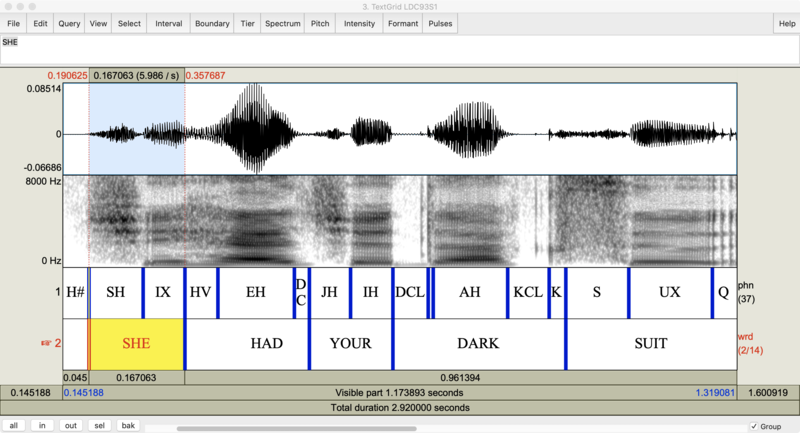
\includegraphics[height=2.5in]{shehadyourdarksuit.png}}}
\end{frame}

\begin{frame}
  \frametitle{How to Use Phonemes, \#2: CSR}

  Suppose you want to transcribe a sequence of words.  You can do that
  by trying to recognize a sequence of phones, restricted to only
  those sequences that form valid sentences:
  \centerline{\href{https://catalog.ldc.upenn.edu/LDC93S1}{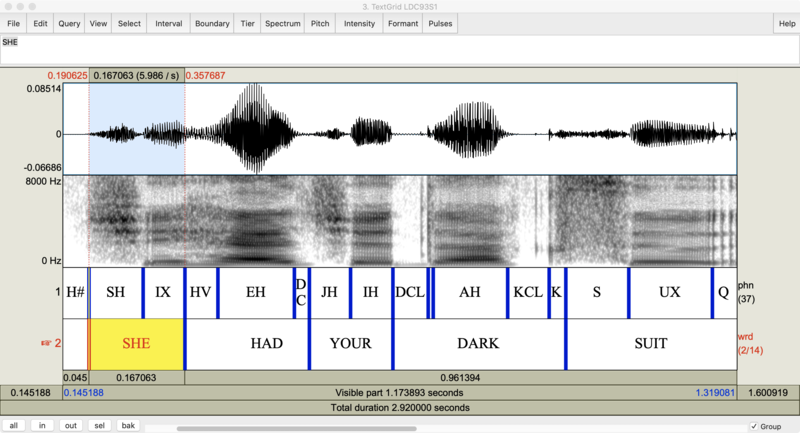
\includegraphics[height=2.5in]{shehadyourdarksuit.png}}}
\end{frame}

\begin{frame}
  \frametitle{How to Use Phonemes, \#2: Large Vocabulary}

  Suppose you have good models of each phoneme.  Now you want to
  recognize the word ``supercalifragilisticexpialidocious.''  No
  problem.  You just create a new word model, by stringing together
  the phoneme models like this:
  \begin{block}{Dictionary entry for ``supercalifragilisticexpialidocious''}
    \ipa{sup{\textrhookrevepsilon}k{\ae}lIfr{\ae}dZIlIstIkEkspi{\ae}lIdoS2s}
  \end{block}
\end{frame}

\begin{frame}
  \frametitle{Generalizing from one language to another}

  \begin{itemize}
  \item Two {\bf phonemes} are different if they distinguish two
    words, e.g., ``bat'' vs. ``pat.''  Therefore, {\bf phonemes are
      language-dependent}.
  \item However, many languages have similar phonemes, e.g., most
    languages have \ipa{/mama/}.
  \item {\bf Phones} are discrete segmental units, like phonemes,
    but not required to be language-dependent.  In fact, we mostly just choose
    a phone set which is most convenient for  our own  software.
  \end{itemize}
\end{frame}

\begin{frame}
  \frametitle{Phones vs.~Phonemes: Example}

  \begin{block}{Two phones that are different phonemes in French, but the same phoneme in English}
    \begin{itemize}
    \item French has the words {\bf ou} (\ipa{[u]}, ``or'') and {\bf eu}
      (\ipa{[y]}, ``had''), that sound like the same vowel in English,
      but are different vowels in French.
    \item The phone \ipa{/y/} (rounded \ipa{/i/}) is not part of the phoneme inventory of English.
      If an English speaker hears it, they think you're saying either \ipa{/u/} or \ipa{/i/}.
    \end{itemize}
  \end{block}

  \begin{block}{Two phones that are different phonemes in English, but the same phoneme in Spanish}
    English has the words {\bf thin} (\ipa{/TIn/}) and {\bf sin}
    (\ipa{/sIn/}).  In Spanish, these sound like two versions of the
    same word ({\bf cien}), pronounced with European vs.~Latin American
    accent, respectively.
  \end{block}
\end{frame}

\begin{frame}
  \frametitle{``Language Independent and Language Adaptive Large
    Vocabulary Speech Recognition,'' Schultz \& Waibel, 1998}
  \centerline{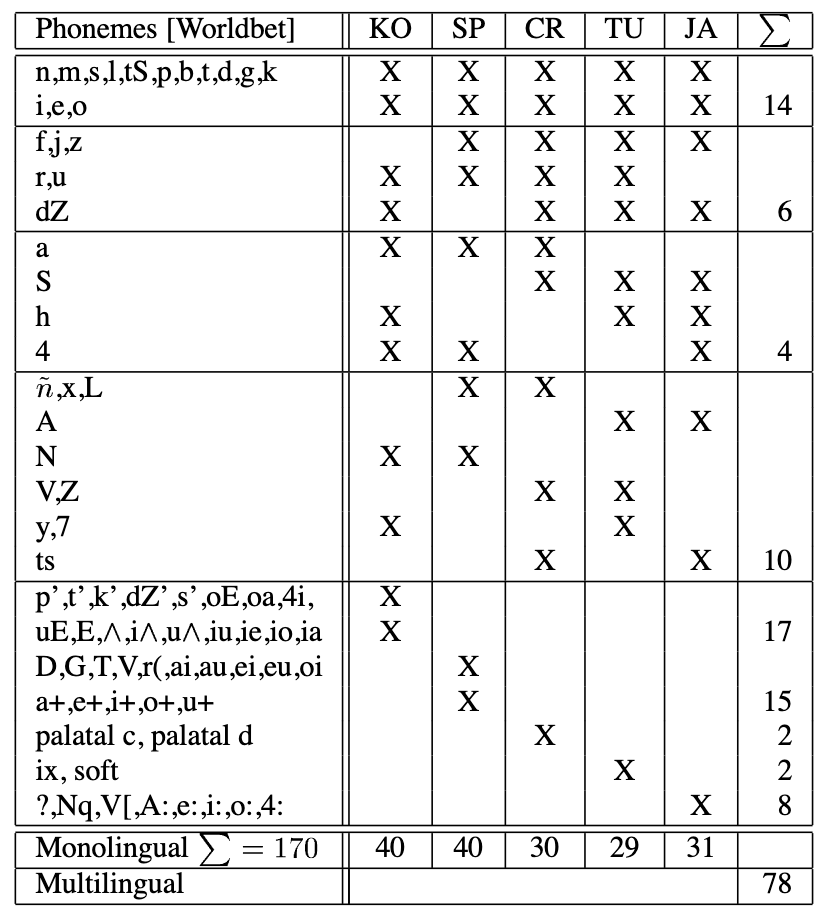
\includegraphics[height=2.9in]{schultz1998.png}}
\end{frame}

%%%%%%%%%%%%%%%%%%%%%%%%%%%%%%%%%%%%%%%%%%%%
\section[Bayesian vs. Discriminative]{Bayesian vs. Discriminative Classifiers}
\setcounter{subsection}{1}

\begin{frame}
  \frametitle{Neural net phone models: Basic setup}

  \begin{itemize}
    \item Start with mel-filterbank or gammatone features, say, 40
      dimensions per frame.  Concatenate 11 frames together, centered
      at frame $t$, and call that $\vec{x}$ (440 dimensions).
    \item Define $q$ to be the ``state'' at time $t$.
      \begin{itemize}
      \item For now we'll say ``state''=''phone,''
        $q\in\left\{1,\ldots,39\right\}$, because there are 39
        phonemes in English.
      \item In a real experimental system, we might subdivide each
        phone into two or three states, each of which has forty or
        fifty context-dependent variants, which would give
        $q\in{\mathcal Q}$ where $|{\mathcal Q}|=39\times 3\times
        50=5850$ or so.
      \end{itemize}
    \item The neural net output is a 39-vector $\hat{y}_t$ such that
      \[
      \hat{y}[i] = p\left(q=i|\vec{x}\right),~~~1\le i\le 39
      \]
  \end{itemize}
\end{frame}

\begin{frame}
  \frametitle{Discriminative Phone Classifier}

  A discriminative phone classifier chooses, in each frame,
  \begin{displaymath}
    q^* = \argmax \hat{y}[q] = \argmax p\left(q|\vec{x}\right)
  \end{displaymath}
  \begin{itemize}
  \item
    That's the optimal thing to do if $\vec{x}$ is the only
    information we have.
  \item
    If we have other information, then $q^* = \argmax \hat{y}[q]$ is
    suboptimal because it ignores our other information.
  \end{itemize}
\end{frame}

\begin{frame}
  \frametitle{Other Sources of Information}

  What other sources of information might we have? Here are two
  possibilities:
  \begin{enumerate}
  \item {\bf Information about Genre:} Maybe the test speech and
    training speech are about different subjects.  In the training
    speech, a particular phoneme (say, $q=k$) never occurs, therefore
    the neural network always gives it a very low probability
    ($q(q=k|\vec{x})\approx 0$), regardless of $\vec{x}$.  We know the
    test genre, so we know that $q=k$ should be much more frequent.
    How can we fix that?
  \item {\bf Information about Sequence:} Maybe we have a language
    model that tells us $p(q|C)$, which is the
    probability of observing phone $q$ after a particular context
    of preceding phones, ($C=(q_1,\ldots,q_{t-1})$).  How can we combine
    $p(q|C)$ with $p\left(q|\vec{x}\right)$?
  \end{enumerate}
\end{frame}

\begin{frame}
  \frametitle{Bayesian Phone Classifier}

  A Bayesian phone classifier fuses information from multiple sources
  using Bayes' rule:
  \begin{displaymath}
    p(q=i|C,\vec{x}) = \frac{p(q=i|C)p(\vec{x}|q=i)}{\sum_j p(q=j|C)p(\vec{x}|q=j)}
  \end{displaymath}
  Then, {\bf after} performing information fusion, we can choose the
  most probable phone:
  \begin{displaymath}
    q^* = \argmax p(q=i|C,\vec{x})
  \end{displaymath}
  Now we have just one problem.  How can we compute $p(\vec{x}|q)$?
\end{frame}

\begin{frame}
  \frametitle{The four Bayesian probabilities}

  A Bayesian classifier is defined if we know any row or column from
  the following table:

  \begin{centering}
    \begin{tabular}{|c|c|}\hline
      \begin{minipage}{2in}
        Probability Mass Functions (pmf) (must be  non-negative and sum up to 1)
      \end{minipage} &
      \begin{minipage}{2in}
        Probability Density Functions (pdf) (must be non-negative, but need not be less than 1)
      \end{minipage} \\ \hline
      \begin{minipage}{2in}
        {\bf Prior:}
        $$p(q)$$
      \end{minipage} &
      \begin{minipage}{2in}
        {\bf Likelihood:}
        $$p(\vec{x}|q)$$
      \end{minipage} \\\hline
      \begin{minipage}{2in}
        {\bf Posterior:}
        $$p(q|\vec{x})$$
      \end{minipage} &
      \begin{minipage}{2in}
        {\bf Evidence:}
        $$p(\vec{x})$$
      \end{minipage} \\\hline
    \end{tabular}\\
  \end{centering}
\end{frame}

%%%%%%%%%%%%%%%%%%%%%%%%%%%%%%%%%%%%%%%%%%%%
\section[Softmax as a Posterior]{How to compute the likelihood if the softmax is a posterior}
\setcounter{subsection}{1}

\begin{frame}
  \frametitle{Why can we interpret  $\hat{y}[i]$ as a posterior?}

  Remember why we can say $\hat{y}[i]=p\left(q=i|\vec{x}\right)$.
  It's because of two things:
  \begin{enumerate}
    \item $\hat{y}$ is trained using MSE for linear outputs (or using
      cross-entropy for softmax outputs, which has the same gradient),
      so, given enough training data, it learns
      \begin{displaymath}
        \hat{y}[i] = E\left[y[i]|\vec{x}\right] = p\left(y[i]=1|\vec{x}\right)
      \end{displaymath}
    \item $\hat{y}$ is computed using a softmax nonlinearity, which
      guarantees that $\hat{y}[i]>0$ and
      \begin{displaymath}
        \sum_{j=1}^{39} \hat{y}[i]=1
      \end{displaymath}
  \end{enumerate}
\end{frame}

\begin{frame}
  \begin{block}{The form of the softmax nonlinearity}
  Remember that we define the softmax as a nonlinear transform from
  some excitation, $e^{(2)}_j$, to its output activation,
  $\hat{y}[j]$.  Let's drop the superscript, so we can write
  \begin{displaymath}
    \hat{y}[i] = \frac{\exp(e[i])}{\sum_{j=1}^{39} \exp(e[j])}.
  \end{displaymath}
  \end{block}

  \begin{block}{Bayes' rule}
    Bayes' rule defines a method for computing $p(q|\vec{x})$ in terms
    of $p(\vec{x}|q)$.  It is
    \begin{displaymath}
      p(q=i|\vec{x}) = \frac{p(q=i,\vec{x})}{\sum_{j=1}^{39} p(q=j,\vec{x})}
    \end{displaymath}
  \end{block}
  Notice the similarity in those two equations.  Can we make use of that?
\end{frame}

\begin{frame}
  \frametitle{Relationship between softmax and Bayes' rule}

  Suppose the neural net has been trained so that
  $\hat{y}[i]=p(q=i|\vec{x})$.  Then we can write
  \begin{displaymath}
    \frac{p(q=i,\vec{x})}{\sum_{j=1}^{39} p(q=j,\vec{x})} =
    \frac{G\exp(e[i])}{G\sum_{j=1}^{39} \exp(e[j])}.
  \end{displaymath}
  The only way this can be true is if
  \begin{displaymath}
    p(q=i,\vec{x}) = G\exp(e[i])
  \end{displaymath}
  for some value of $G$.  The only problem: we have no idea what $G$
  is.  We have to be a little careful in our derivations, but usually
  we can just choose some value with good numerical properties, like
  $G=1/\max_j \exp(e[j])$ for example.
\end{frame}

\begin{frame}
  \frametitle{Bayesian probabilities and Neural nets}
  Here's how we can estimate the four Bayesian probabilities using a neural net:
  \begin{enumerate}
  \item {\bf Prior:}
    \begin{displaymath}
      p(q=i) = \frac{\mbox{\# times $q=i$ occurred in training data}}{\mbox{\# frames in training data}}
    \end{displaymath}
  \item {\bf Posterior:}
    \begin{displaymath}
      p(q=i|\vec{x}) = \softmax\left(e[i]\right)
    \end{displaymath}
  \end{enumerate}
\end{frame}

    
\begin{frame}
  \frametitle{Bayesian probabilities and Neural nets}
  Here's how we can estimate the four Bayesian probabilities using a neural net:
  \begin{enumerate}
  \item {\bf Evidence:}
    \begin{displaymath}
      p(\vec{x}) = G\sum_j\exp(e[j])
    \end{displaymath}
    for some unknown value of $G$.
  \item {\bf Likelihood:}
    \begin{displaymath}
      p(\vec{x}|q=i) = \frac{G\exp(e[i])}{p(q=i)}
    \end{displaymath}
  \end{enumerate}
  We have to be a little careful in our derivations, but usually we
  can just choose some value of $G$ with good numerical properties,
  like $G=1/\max_j \exp(e[j])$ for example.
\end{frame}

\begin{frame}
  \frametitle{Why the likelihood is useful}

  \begin{enumerate}
  \item {\bf Train-test mismatch}.  Suppose that some particular phone
    ($q=i$, say) was almost never seen in training data, but it might
    occur sometimes in test data.
    \begin{itemize}
    \item $p(q=i|\vec{x})\approx 0$, because it was never seen in
      training data. If you classify using $q^*=\argmax p(q|\vec{x})$,
      it will never get recognized.
    \item $p(q=i)\approx 0$ is also very small. Therefore
      $$p(\vec{x}|q=i) = \frac{G\exp(e[i])}{p(q=i)}$$ might be
      reasonably-sized, and might sometimes get recognized.
    \end{itemize}
  \item {\bf Information fusion}.  Suppose you have a language model
    that tells you $p(q|C)$, the probability of $q$ given some context
    variable $C$.  Then
    \begin{displaymath}
      p(q,\vec{x}|C) = p(\vec{x}|q)p(q|C)
    \end{displaymath}
  \end{enumerate}
\end{frame}

%%%%%%%%%%%%%%%%%%%%%%%%%%%%%%%%%%%%%%%%%%%%
\section[Summary]{Where we're going next}
\setcounter{subsection}{1}

\begin{frame}
  \frametitle{Summary: Neural Nets and Probability}

  The two most important Bayesian probabilities are
  \begin{itemize}
  \item {\bf Posterior:} This is what you want if there is no
    train-test mismatch, and if you don't need to do information
    fusion.  It is given by
    \begin{displaymath}
      p(q=i|\vec{x})=\softmax(e[i]) = \frac{\exp(e[i])}{\sum_j \exp(e[j])}
    \end{displaymath}
  \item {\bf Likelihood:} This is what you want if there is train-test
    mismatch, or if you need to fuse information from two or more
    different sources.  It is given by
    \begin{displaymath}
      p(\vec{x}|q=i) = \frac{G\exp(e[i])}{p(q=i)}
    \end{displaymath}
    where $G$ is an unknown constant.  
    We have to be a little careful in our derivations, but usually we
    can just choose some value of $G$ with good numerical properties,
    like $G=1/\max_j \exp(e[j])$ for example.
  \end{itemize}
\end{frame}

\begin{frame}
  \frametitle{Where We're Going Next: Information Fusion}

  Next time, we will talk about a particular type of context
  information: the pronunciation model and language model, in the form
  of a hidden Markov model.
\end{frame}

\end{document}

